\question{Câu 10}

Cho mạch khuếch đại tín hiệu như hình vẽ. Mạch có $V_{CC}=9V$. BJT $Q_{1}$ và $Q_{2}$ có hệ số $\beta = 100$. Các hệ số $V_{A} = \infty$.

\begin{figure}[H]
	\centering
	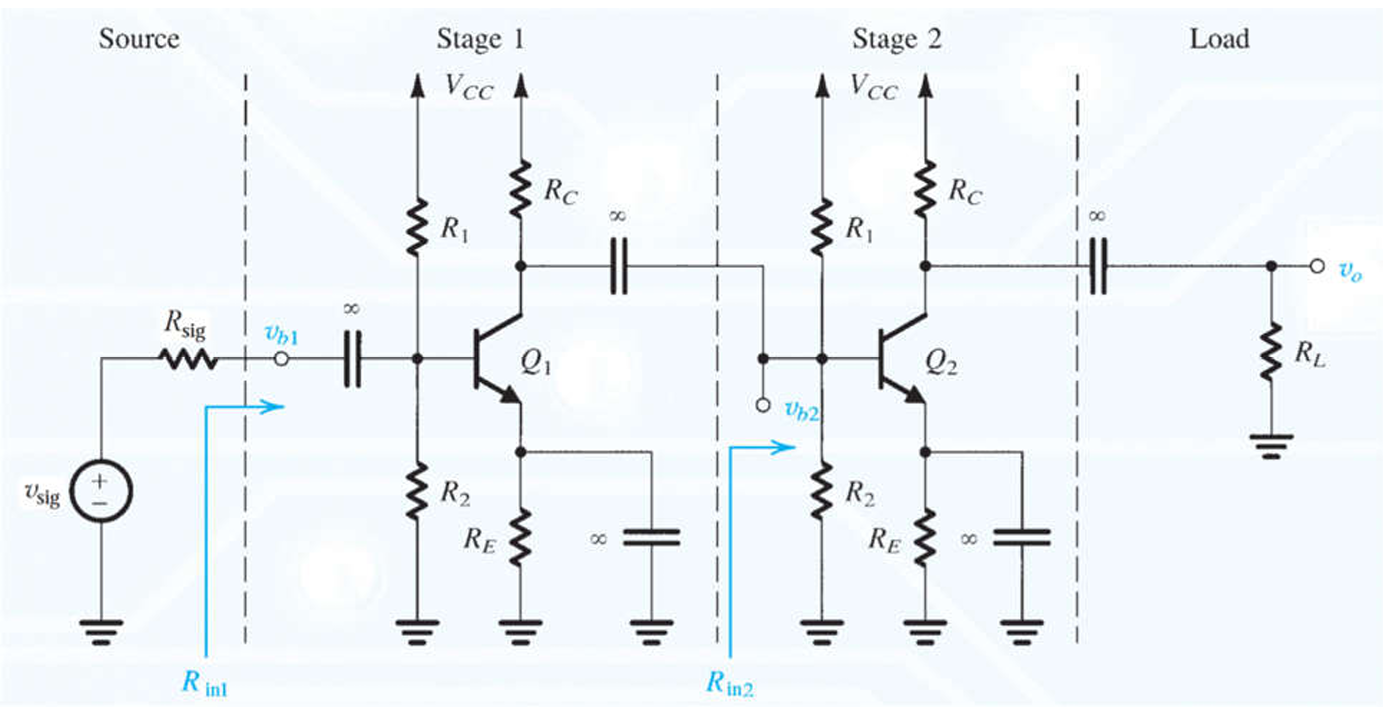
\includegraphics[width=.8\linewidth]{./my-chapters/my-images/Question10/Debai.png}
\end{figure}

\answer{a}{Thiết kế để có $Q_{1}(0.5mA\text{, }6V)$, $Q_{2}(2mA\text{, }6V)$}

\begin{itemize}[label=-]
	\item Xét tầng 1 (SWEEP bf cho đến khi thỏa điểm Q)

\begin{figure}[H]
	\centering
	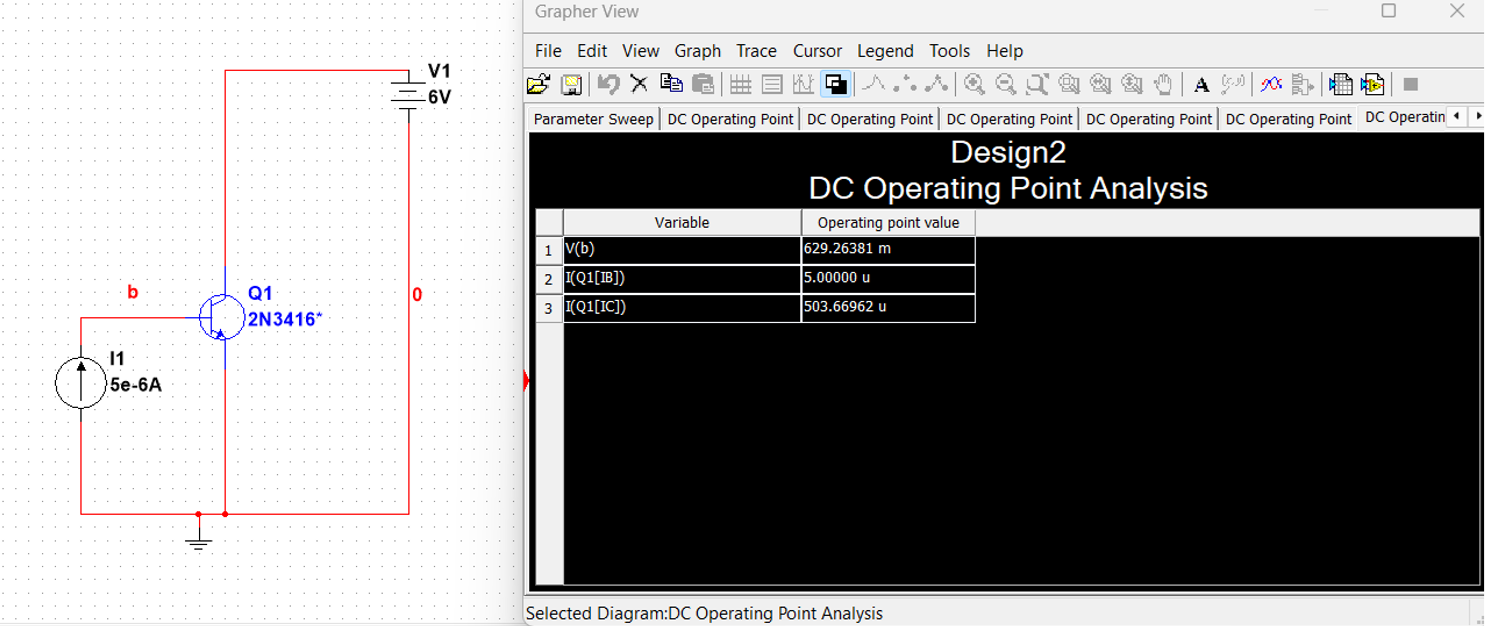
\includegraphics[width=\linewidth]{./my-chapters/my-images/Question10/a_tang1.png}
	\caption{Chọn trasistor $Q_{1}$ thỏa mãn $\beta = 100$ ứng với $I_{C1}= 0.5 mA$ và $V_{CE1} = 6V$ (chọn \textbf{NPN 2N3416} với thông số bf chỉnh thấp còn 140 so với 157 ban đầu); $V_{BE1} = 0.63 V$}
\end{figure}

\noindent Ta có: $Q_1( I_{CQ1} = 0.5{mA},\; V_{CEQ1} = 6{V})$

Ta có:
\[
R_{TH1} = R_1 // R_2 \tag{1}
\]
\[
V_{TH1} = \frac{R_2}{R_1 + R_2} V_{CC} \tag{2}
\]

Từ phương trình mạch:
\[
V_{CC} - V_{CEQ1} = I_{CQ1}(R_C + R_E)
\]
\[
\Rightarrow 9 - 6 = 0.5(R_C + R_E)
\]
\[
\Rightarrow R_C + R_E = 6\,\text{k}\Omega \tag{3}
\]

Công thức dòng collector:
\[
I_{CQ1} = \frac{(V_{TH1} - V_{BE1})\beta}{R_{TH1} + (\beta + 1)R_E} \tag{4}
\]
Chọn \( R_{TH1} \ll (\beta + 1)R_E \) để dòng \( I_C \) ổn định.  

Giả sử chọn:
\[
R_E = 2\,\text{k}\Omega \Rightarrow R_{TH1} \ll 202\,\text{k}\Omega \Rightarrow R_{TH1} = 20.2\,\text{k}\Omega
\]

Thế \( R_{TH1} \) và \( R_E \) vào (4), ta được:
\[
V_{TH1} = 1.741\,\text{V}
\]

Từ (3):
\[
R_C = 4\,\text{k}\Omega
\]

Từ (2):
\[
\frac{R_2}{R_1 + R_2} = 0.1934 \quad \Rightarrow \quad 4.17R_2 = R_1
\]

Lại có:
\[
R_1 // R_2 = 20.2\,\text{k}\Omega
\]
\[
\Rightarrow R_2 = 25\,\text{k}\Omega,\quad R_1 = 104.25\,\text{k}\Omega
\]

\begin{figure}[H]
	\centering
	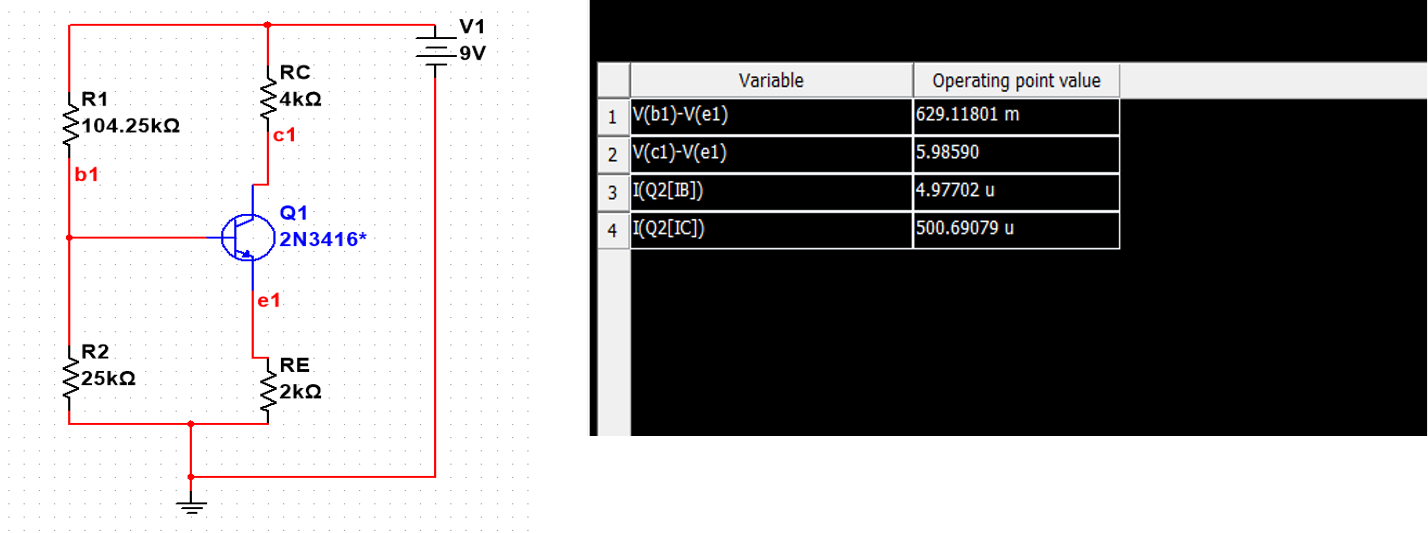
\includegraphics[width=.9\linewidth]{./my-chapters/my-images/Question10/a_tang2.png}
	\caption{Mạch Bias cho tầng 1 và mô phỏng điểm Q tầng 1}
\end{figure}

\item Xét tầng 2 (SWEEP bf cho đến khi thỏa điểm Q)

\begin{figure}[H]
	\centering
	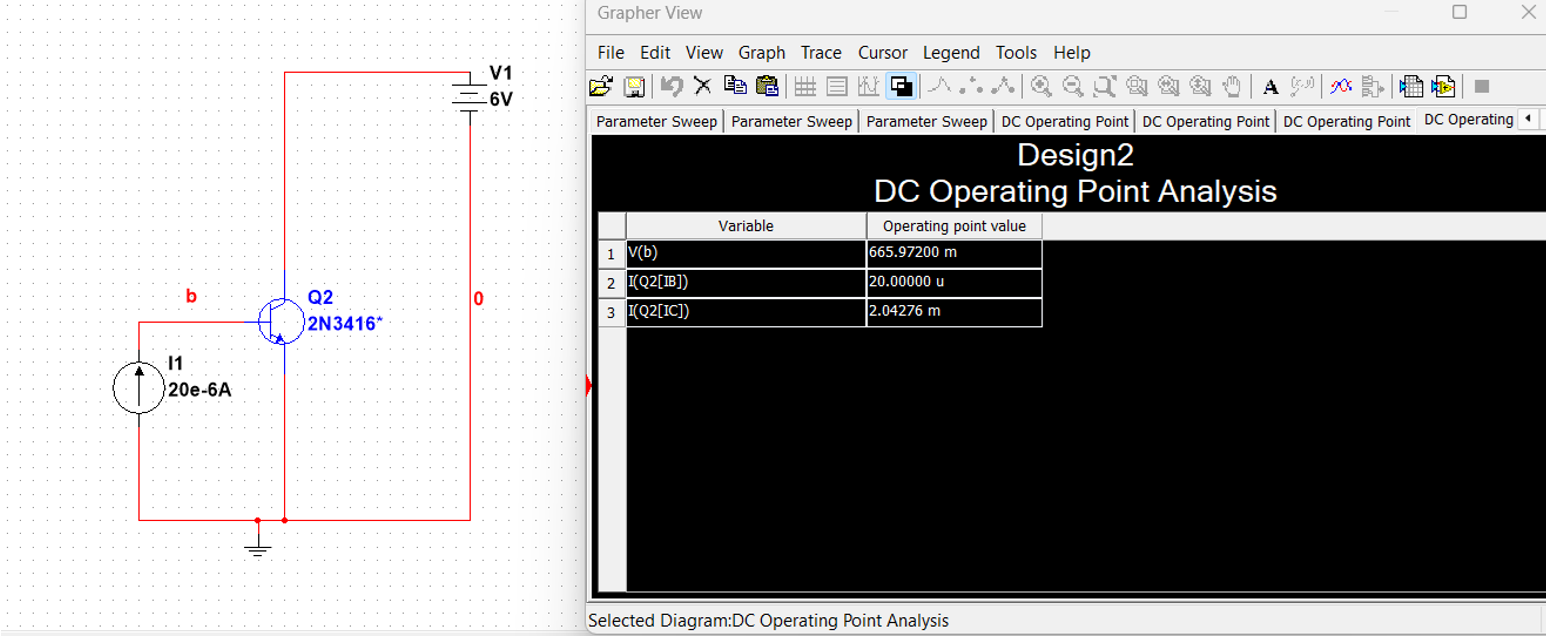
\includegraphics[width=.8\linewidth]{./my-chapters/my-images/Question10/a_tang3.png}
	\caption{Chọn trasistor $Q_{2}$ thỏa mãn $\beta = 100$ ứng với $I_{C2} = 2 mA$ và $V_{CE2} = 6V$ (chọn \textbf{NPN 2N3416} với thông số bf chỉnh thấp còn 112 so với 157 ban đầu); $V_{BE2} =0.665V$.}
\end{figure}

\noindent Ta có: $Q_2( I_{CQ2} = 2{mA},\; V_{CEQ2} = 6{V})$

Ta có:
\[
R_{TH2} = R_1 // R_2 \tag{1}
\]
\[
V_{TH2} = \frac{R_2}{R_1 + R_2} V_{CC} \tag{2}
\]

Phương trình mạch:
\[
V_{CC} - V_{CEQ2} = I_{CQ2}(R_C + R_E)
\]
\[
\Rightarrow 9 - 6 = 2(R_C + R_E)
\]
\[
\Rightarrow R_C + R_E = 1.5\,\text{k}\Omega \tag{3}
\]

Công thức dòng collector:
\[
I_{CQ2} = \frac{(V_{TH2} - V_{BE2})\beta}{R_{TH2} + (\beta + 1)R_E} \tag{4}
\]
Chọn \( R_{TH2} \ll (\beta + 1)R_E \) để dòng \( I_C \) ổn định.  

Giả sử chọn: \finalresult{R_E = 500\,\Omega}
\[
\Rightarrow R_{TH2} \ll 50.5\,\text{k}\Omega \Rightarrow R_{TH2} = 5.05\,\text{k}\Omega
\]

Thế \( R_{TH2} \) và \( R_E \) vào (4), ta được:
\[
V_{TH2} = 1.776\,\text{V}
\]

Từ (3):

\finalresult{R_C = 1\,\text{k}\Omega}

Từ (2):
\[
\frac{R_2}{R_1 + R_2} = 0.1973 \quad \Rightarrow \quad 4.07R_2 = R_1
\]

Lại có:
\[
R_1 // R_2 = 5.05\,\text{k}\Omega
\]

$\Rightarrow$ \finalresult{R_2 = 6.3\,\text{k}\Omega} 

$\Rightarrow$ \finalresult{R_1 = 25.6\,\text{k}\Omega}

\begin{figure}[H]
	\centering
	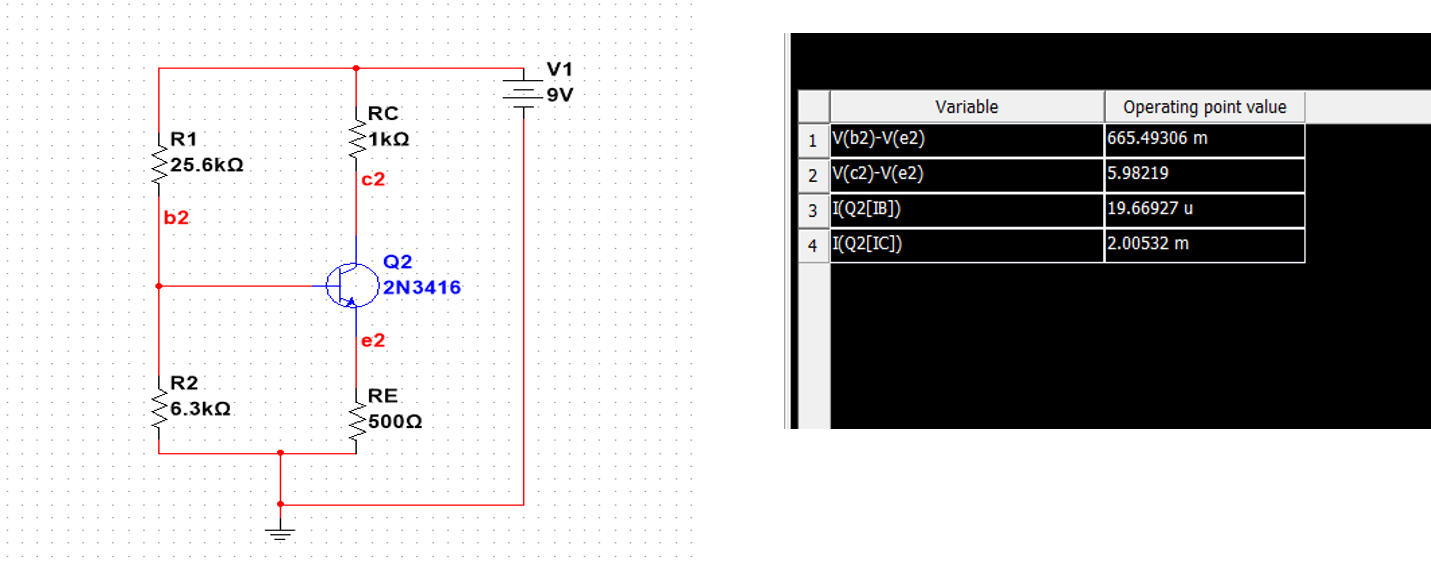
\includegraphics[width=.8\linewidth]{./my-chapters/my-images/Question10/a_tang4.png}
	\caption{Mạch Bias cho tầng 2 và mô phỏng điểm Q tầng 2}
\end{figure}

\end{itemize}

\answer{b}{Đặt nguồn $v_{s} = V_{m} \sin \left(\omega t\right)$ có nội trở $R_{S} = 100k\Omega$ vào mạch. Ngõ ra nối với tải $R_{L}=1k\Omega$. Tìm $A_{vo}$, $A_{v}$, $G_{v}$, $R_{in}$, $R_{out}$ của mạch.}

\begin{figure}[H]
	\centering
	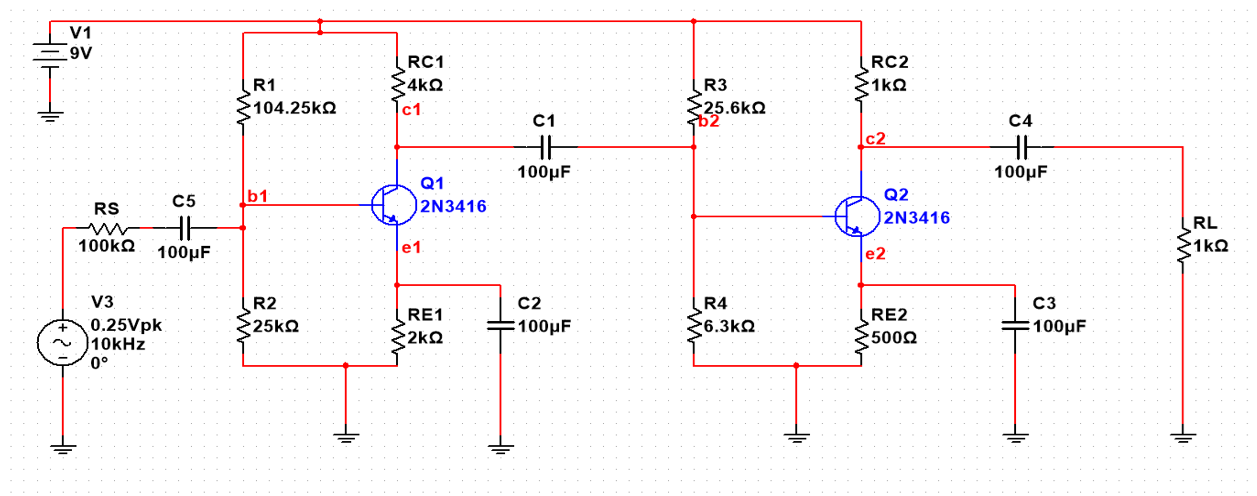
\includegraphics[width=\linewidth]{./my-chapters/my-images/Question10/b_de.png}
\end{figure}

\begin{figure}[H]
	\centering
	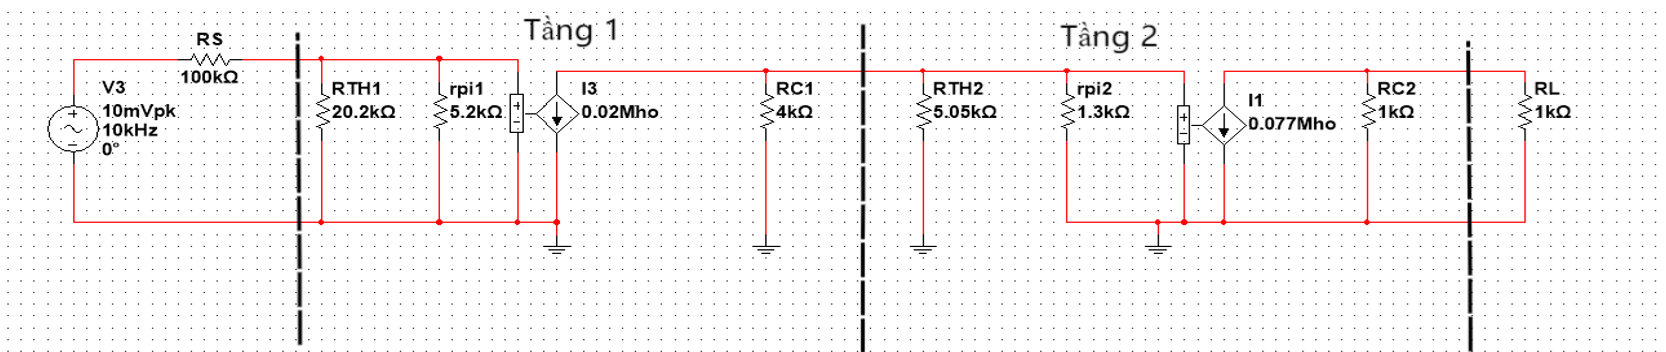
\includegraphics[width=\linewidth]{./my-chapters/my-images/Question10/b_tang.png}
	\caption{mô hình tín hiệu nhỏ.}
\end{figure}

\begin{itemize}[label=-]
	\item Các thông số cơ bản:
	\[
	r_{\pi 1} = \frac{V_T}{I_{B1}} = \frac{V_T \times \beta}{I_{CQ1}}
	= \frac{26 \times 100}{0.5} = 5.2\,\text{k}\Omega
	\]
	\[
	r_{\pi 2} = \frac{V_T}{I_{B2}} = \frac{V_T \times \beta}{I_{CQ2}}
	= \frac{26 \times 100}{2} = 1.3\,\text{k}\Omega
	\]
	\[
	g_{m1} = \frac{I_{CQ1}}{V_T} = \frac{0.5}{26} = 0.02\,(\text{S})
	\]
	\[
	g_{m2} = \frac{I_{CQ2}}{V_T} = \frac{2}{26} = 0.077\,(\text{S})
	\]
	
	\item Tại tầng 1:
	\[
	R_{in1} = R_{TH1} // r_{\pi1}
	= 20.2\,\text{k} // 5.2\,\text{k}
	= 4\,\text{k}\Omega
	\]
	\[
	R_{out1} = R_{C1} = 4\,\text{k}\Omega
	\]
	\[
	A_{V1} = -g_{m1} \times R_{C1}
	= -0.02 \times 4\,\text{k}
	= -80\,(\text{V/V})
	\]
	
	\item Tại tầng 2:
	\[
	R_{in2} = R_{TH2} // r_{\pi2}
	= 5.05\,\text{k} // 1.3\,\text{k}
	= 1.03\,\text{k}\Omega
	\]
	\[
	R_{out2} = R_{C2} = 1\,\text{k}\Omega
	\]
	\[
	A_{V2} = -g_{m2} \times R_{C2}
	= -0.077 \times 1\,\text{k}
	= -77\,(\text{V/V})
	\]
	
	\item Tính $ A_{vo}$, $A_{v}$, $R_{in}$, $R_{out}$ cho toàn bộ mạch
	
	$\Rightarrow$ \finalresult{R_{in} = R_{in1} = 4\,\text{k}\Omega}.
	
	$\Rightarrow$ \finalresult{R_{out} = R_{out2} = 1\,\text{k}\Omega}.
	\[
	A_{v0} = A_{V1} \times A_{V2} \times
	\frac{R_{in2}}{R_{out1} + R_{in2}}
	= (-80) \times (-77) \times
	\frac{1.03}{4 + 1.03}
	= 1261\,(\text{V/V})
	\]
	$\Rightarrow$ \finalresult{A_{v0} = 1261\,(\text{V/V})}.
	\[
	A_v = A_{v0} \times
	\frac{R_L}{R_{out} + R_L}
	= 1261 \times
	\frac{1}{1 + 1}
	= 630.7\,(\text{V/V})
	\]
	$\Rightarrow$ \finalresult{A_{v} = 630.7\,(\text{V/V})}.
	\[
	G_v = A_v \times
	\frac{R_{in}}{R_{in} + R_S}
	= 630.7 \times
	\frac{4}{4 + 100}
	= 24.2\,(\text{V/V})
	\]
	$\Rightarrow$ \finalresult{G_{v} = 24.2\,(\text{V/V})}
	\item Kết quả đo thực nghiệm:
	\begin{figure}[H]
		\centering
		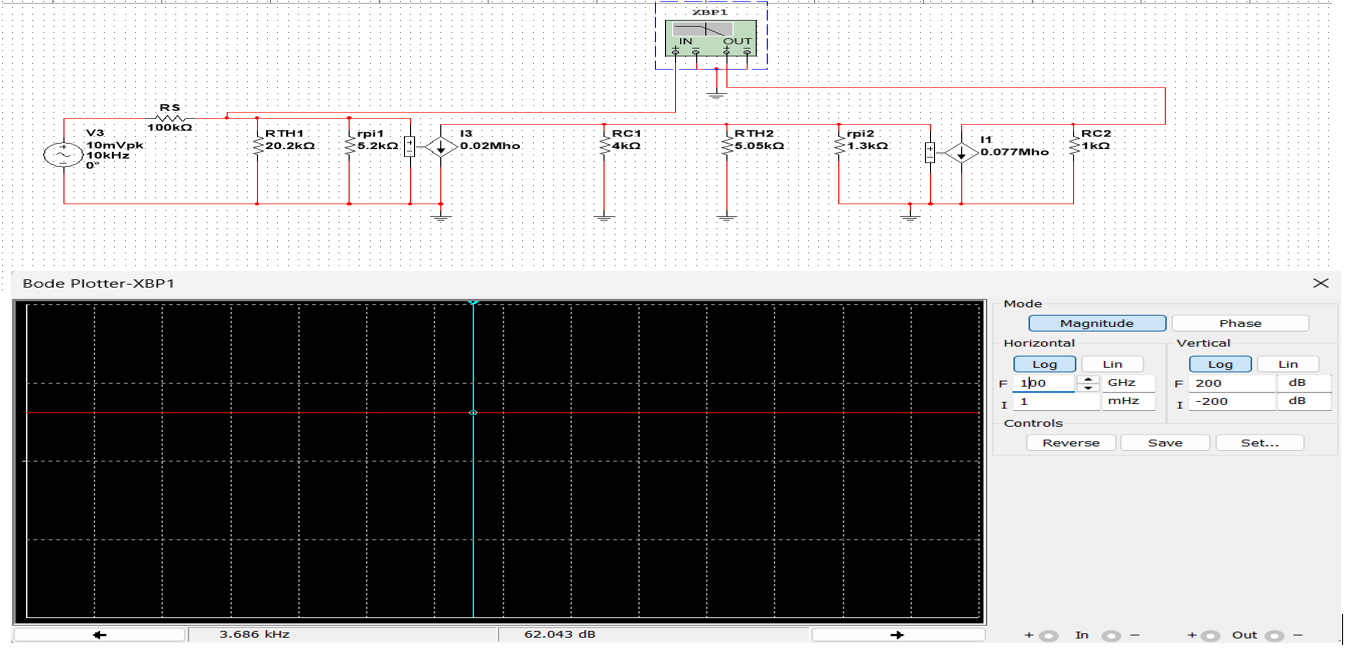
\includegraphics[width=.8\linewidth]{./my-chapters/my-images/Question10/b_ketqua_0.png}
		\caption{Đo $A_{vo} = 62.043db = 1258 V/V$ (mô hình tương đương).}
	\end{figure}
	\begin{figure}[H]
		\centering
		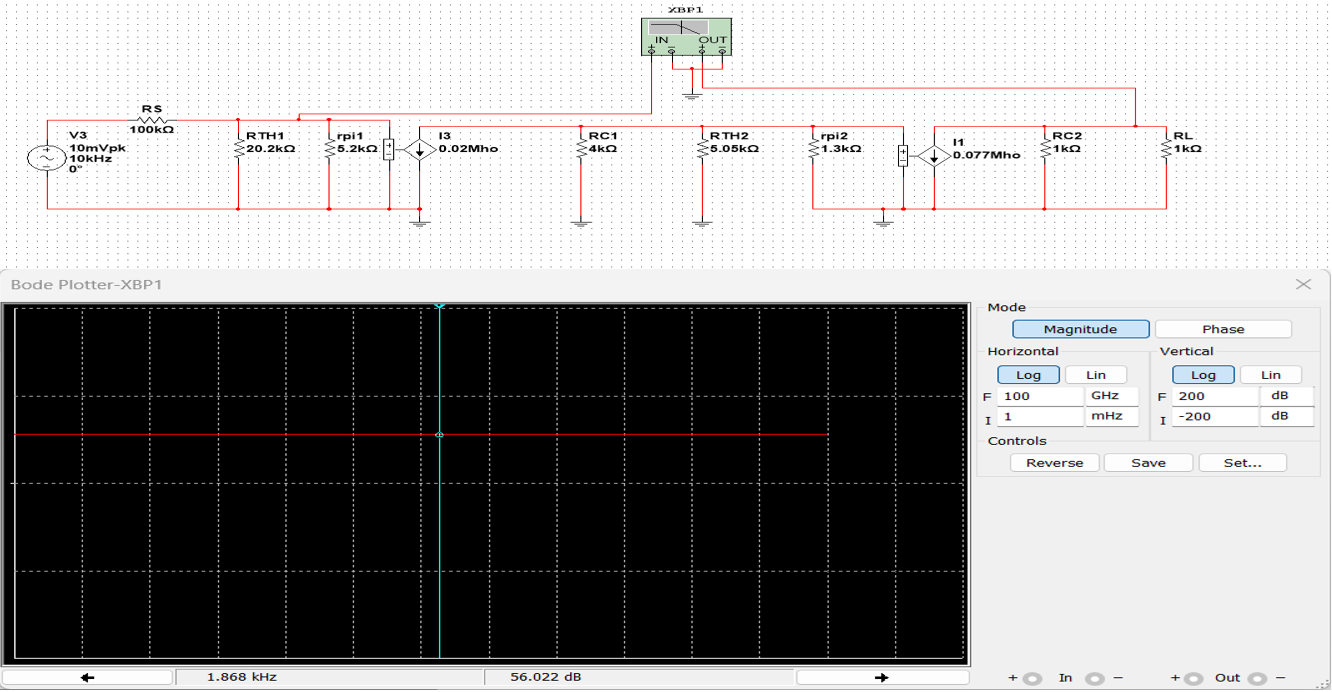
\includegraphics[width=.8\linewidth]{./my-chapters/my-images/Question10/b_ketqua_1.png}
		\caption{Đo $A_{v} = 56 .022 db =  632.55 V/V$ (mô hình tương đương).}
	\end{figure}
	\begin{figure}[H]
		\centering
		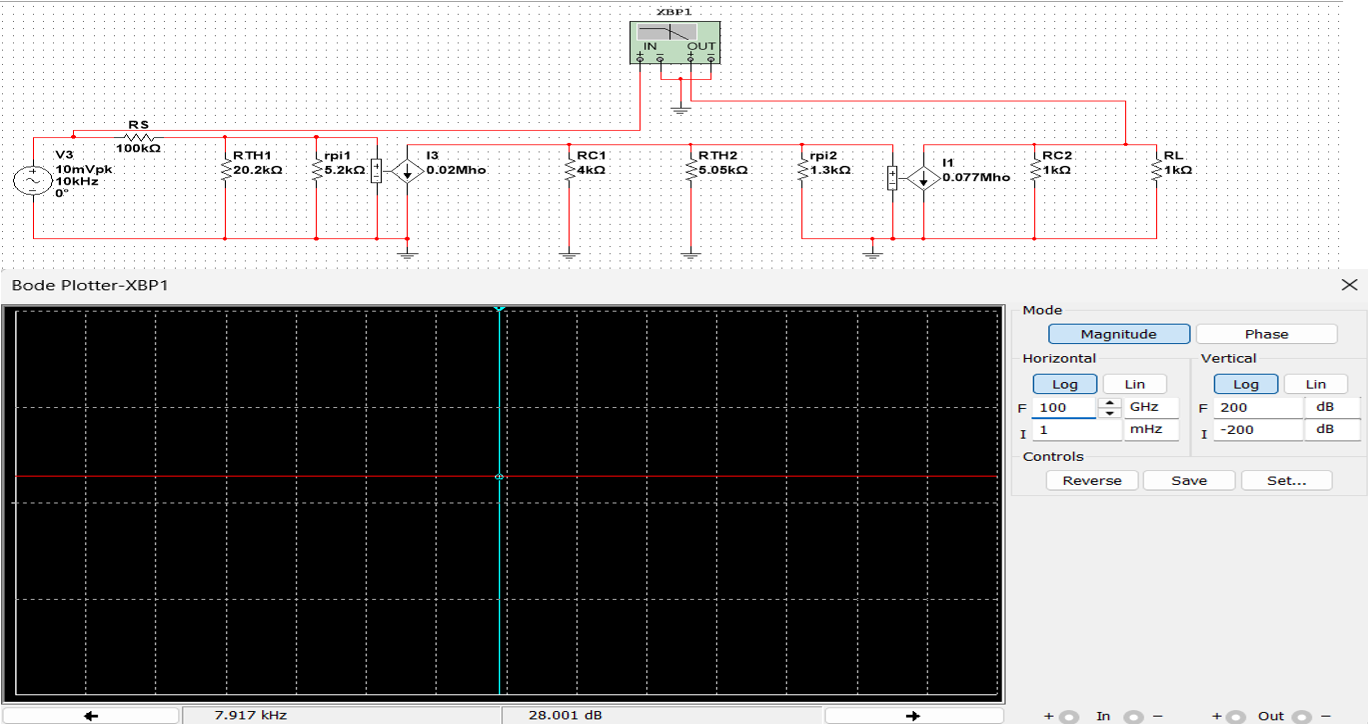
\includegraphics[width=.8\linewidth]{./my-chapters/my-images/Question10/b_ketqua_2.png}
		\caption{Đo $G_{v} = 28 db =  25.11 V/V$ (mô hình tương đương).}
	\end{figure}
	\begin{figure}[H]
		\centering
		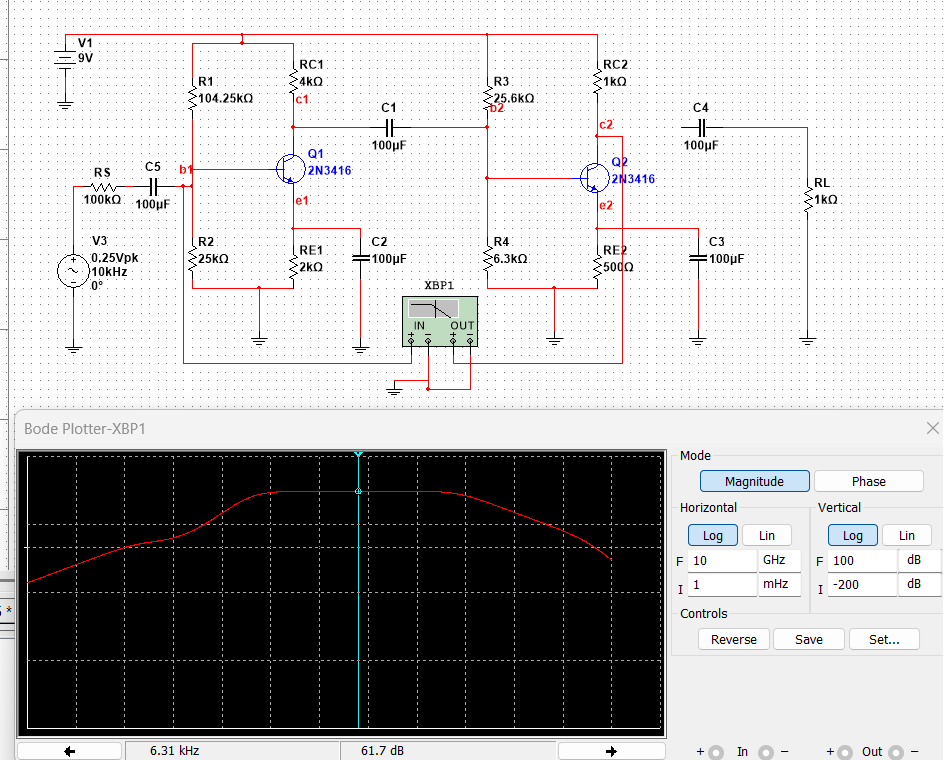
\includegraphics[width=.8\linewidth]{./my-chapters/my-images/Question10/b_ketqua_3.png}
		\caption{Đo $A_{vo} = 61.7db = 1216 V/V$ (toàn mạch).}
	\end{figure}
	\begin{figure}[H]
		\centering
		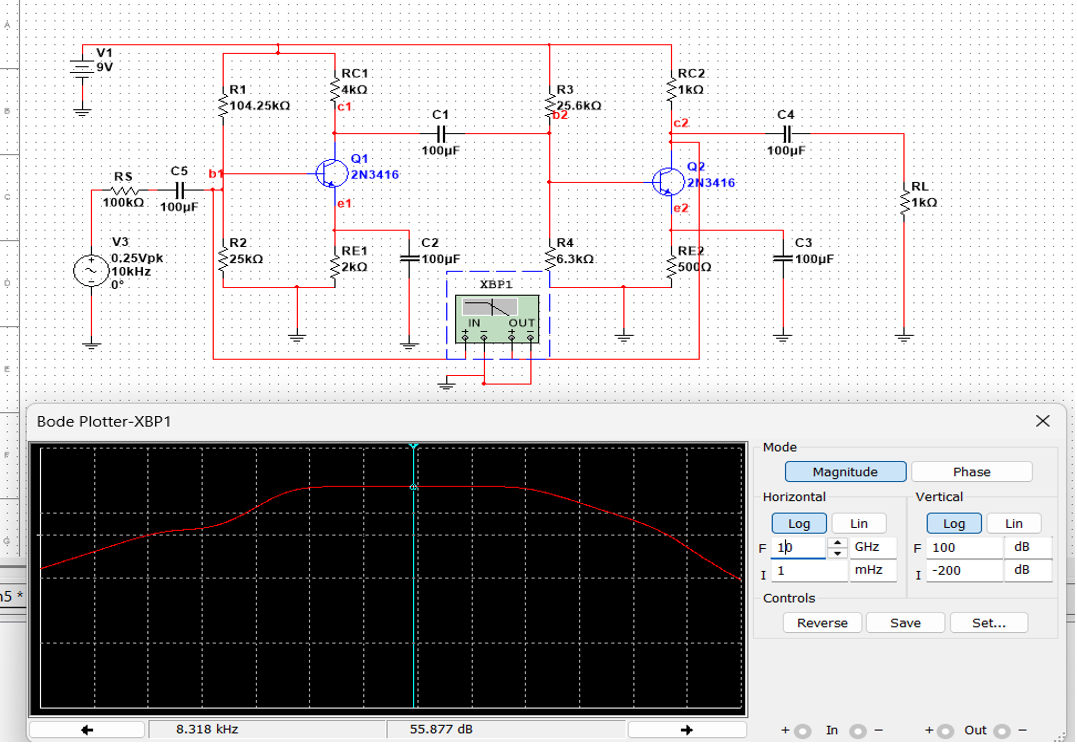
\includegraphics[width=.8\linewidth]{./my-chapters/my-images/Question10/b_ketqua_4.png}
		\caption{Đo $A_{v} = 55.877db = 622.08 V/V$ (toàn mạch).}
	\end{figure}
	\begin{figure}[H]
		\centering
		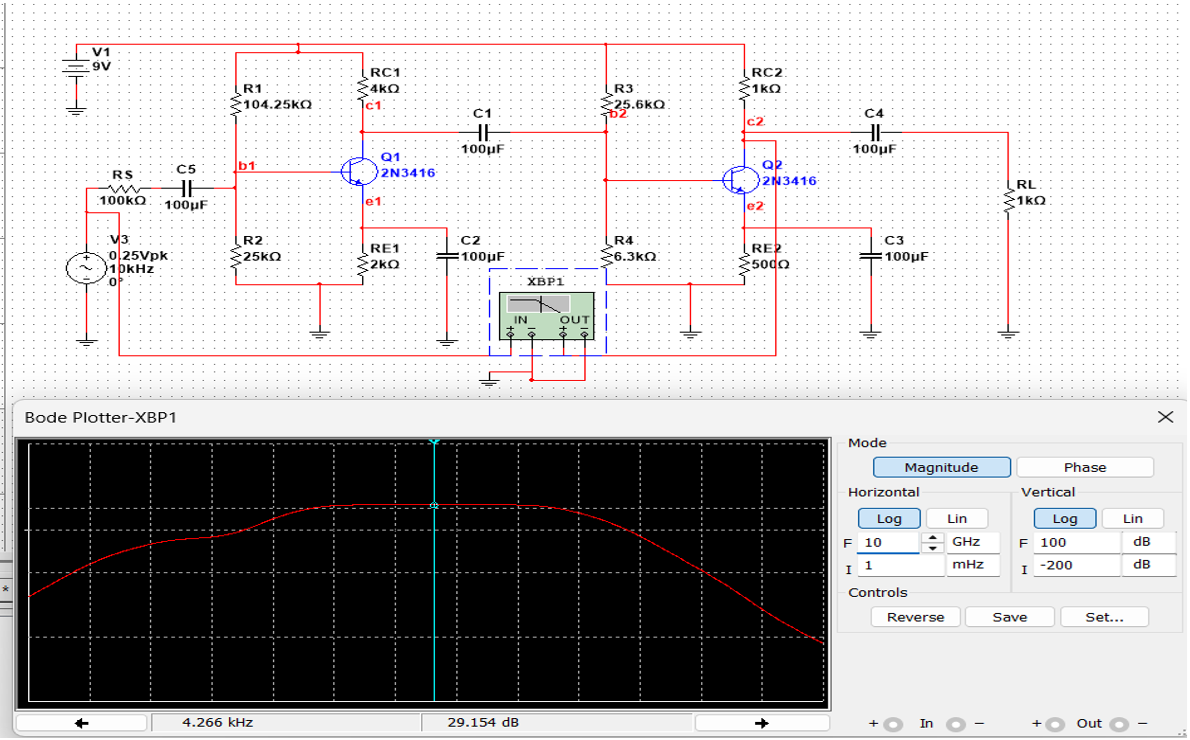
\includegraphics[width=.8\linewidth]{./my-chapters/my-images/Question10/b_ketqua_5.png}
		\caption{Đo $G_{v} = 29.154db = 28.69V/V$  tại tần số $4.266 kHz$( toàn mạch).}
	\end{figure}
\end{itemize}

\answer{c}{Tìm biên độ lớn nhất của $V_{m}$ để để $v_{s}$ là tín hiệu nhỏ ở cả hai tầng.}

Xét Q2 ta có:
\begin{itemize}[label=-]
	\item DC load line: $V_{CE} = V_{CC} - I_{C}(R_{C2} + R_{E2}) \quad \rightarrow \quad V_{CE} = 9 - I_{C} \times 6$
	\item Ac load line: $v_{ce} = -i_{c} ( R_{C2} // R_{L})  →  v_{ce} = -i_{c} \times 0.5$   và đường này cũng phải cắt qua điểm $I_{CQ2}$, được mô tả như hình dưới đây.
\end{itemize}

\begin{figure}[H]
	\centering
	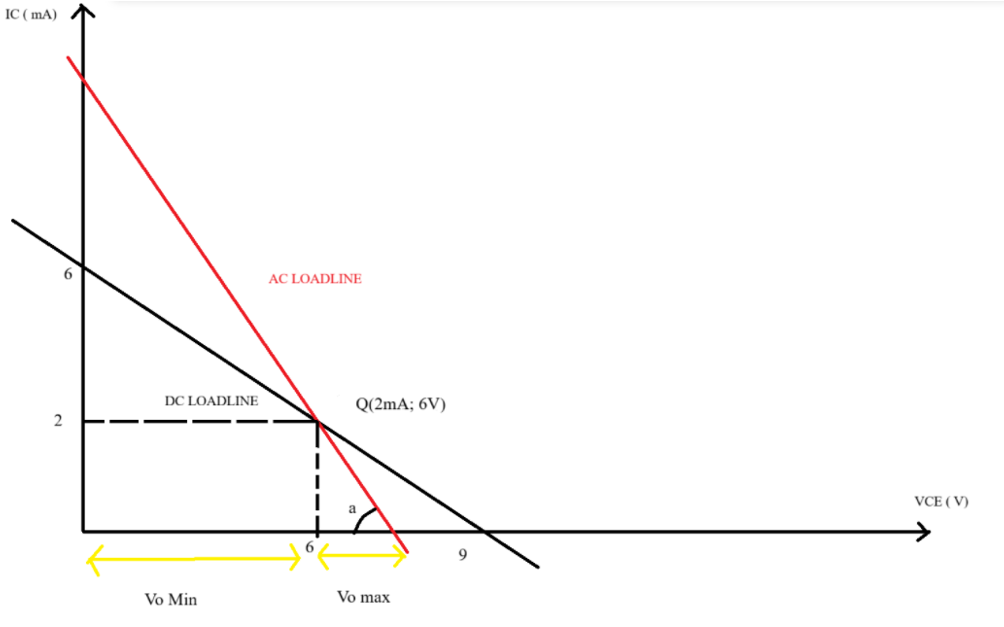
\includegraphics[width=.8\linewidth]{./my-chapters/my-images/Question10/c_hinh.png}
\end{figure}

\[
\tan(\alpha) = \frac{1}{R_L // R_C}
= \frac{1}{0.5\,\text{k}\Omega}
\]

\[
\Rightarrow V_{o_{\text{max}}}
= \frac{I_{CQ2}}{\tan(\alpha)}
= 1\,\text{V}
\]

\[
\Rightarrow V_{\text{sig(max)}}
= \frac{V_{o_{\text{max}}}}{G_V(f = 4.266\,\text{kHz})}
= \frac{1}{28.69}
= 34\,\text{mV}
\]

$\Rightarrow$ \finalresult{V_{\text{sig(max)}} = 34 \,\text{mV}}.

\begin{figure}[H]
	\centering
	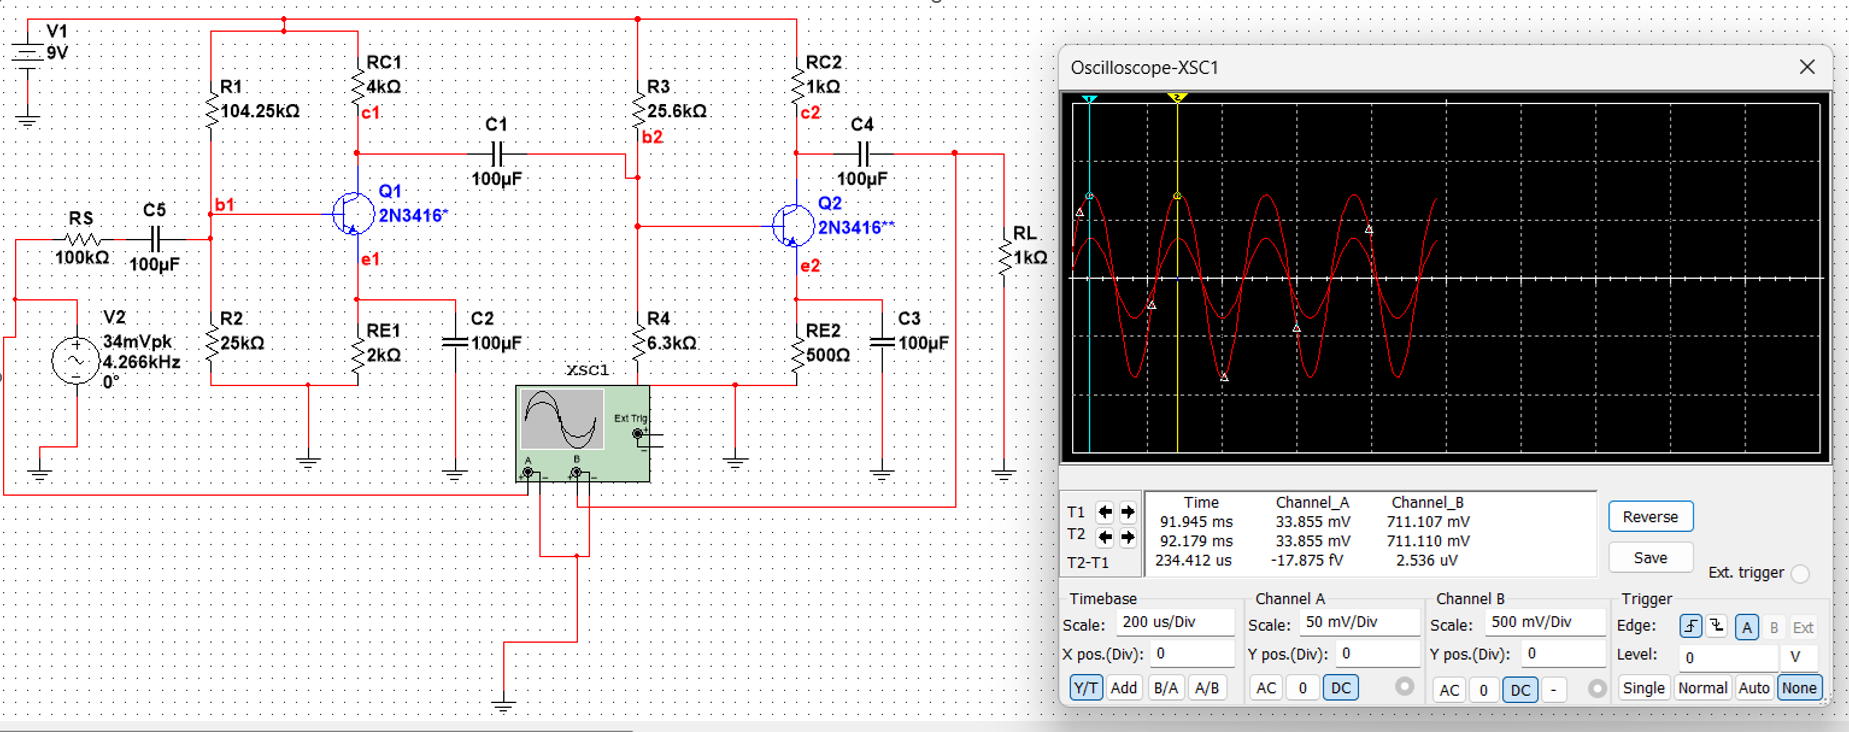
\includegraphics[width=.8\linewidth]{./my-chapters/my-images/Question10/c_ketqua_0.png}
	\caption{$V_{p_{sig}} =34mV$; $V_{p_{L}} = 711 mV$; $G_{v} = 21.54 V/V$.}
\end{figure}
\begin{figure}[H]
	\centering
	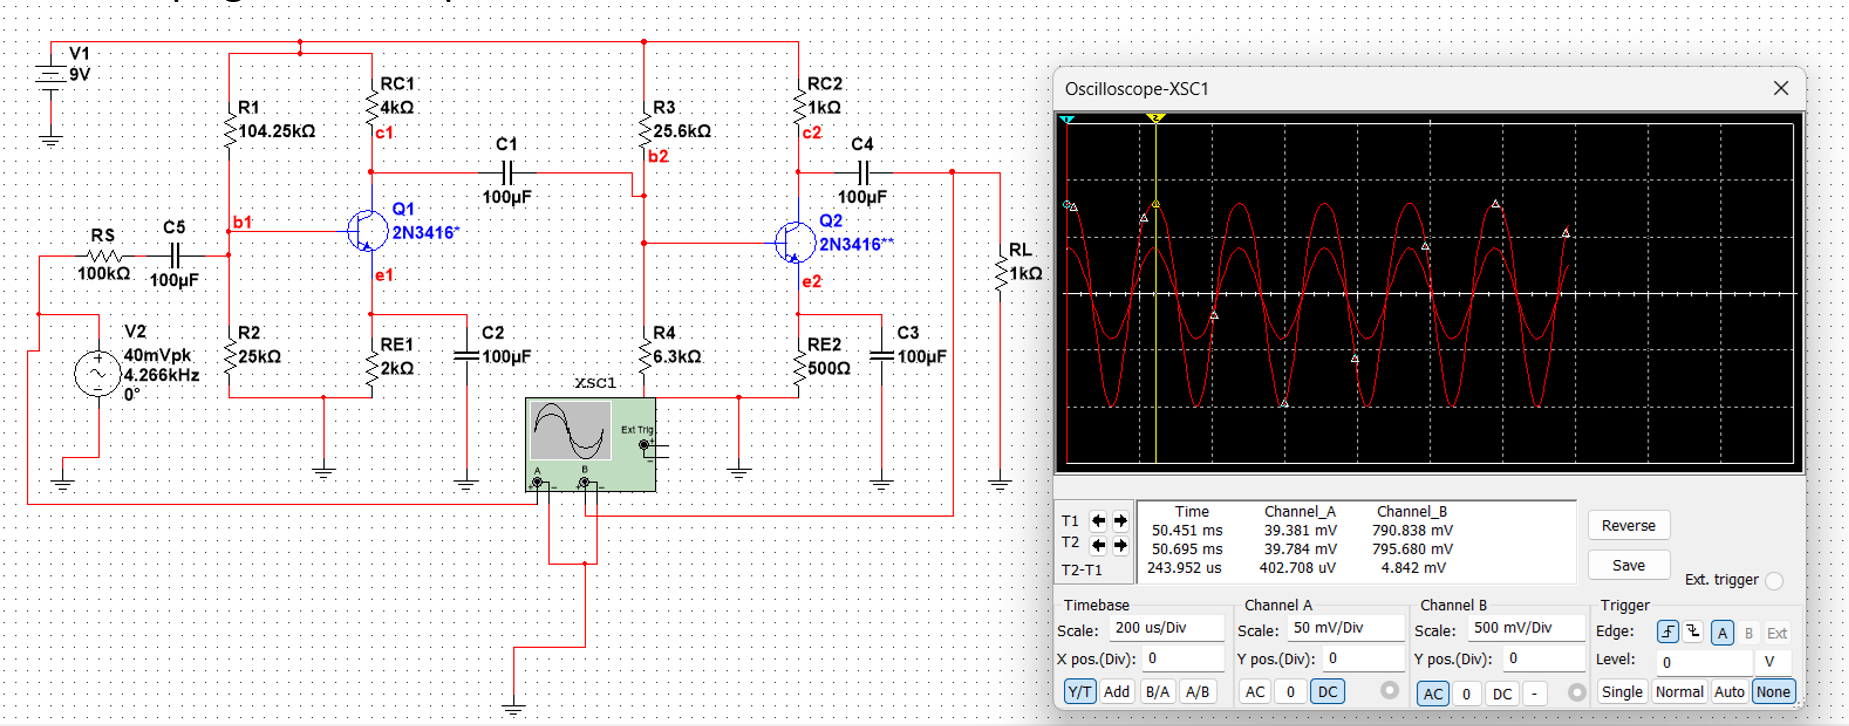
\includegraphics[width=.8\linewidth]{./my-chapters/my-images/Question10/c_ketqua_1.png}
	\caption{$V_{p_{sig}} =40mV$; $V_{p_{L}} = 790.68 mV$; $G_{v} = 19.767V/V$.}
\end{figure}